\section{Grundlagen}
In diesem Abschnitt werden einige grundlegende Elemente erläutert, 
die für das Verständnis der Funktionsweise des Shor-Algorithmus erforderlich sind.
Als Grundfundament sind Kenntnisse in der Modulararithmetik, lineare Algebra und den komplexen Zahlen Vorraussetzung. 

Vorkenntnisse über die Grundprinzipien der Quantenmechanik sind hilfreich, 
werden aber im folgenden Abschnitt erläutert. 


\subsection{RSA-Verschlüsselung}
Das RSA-Verfahren ist ein weitverbreitetes asymmetrisches Kryptosystem, 
das 1977 von Ron \textbf{R}ivest, Adi \textbf{S}hamir und Leonard \textbf{A}dleman entwickelt wurde~\cite{10.1145/359340.359342}. 
In asymmetrischen Verschlüsselungsverfahren werden zwei verschiedene Schlüssel verwendet: 
Ein öffentlicher Schlüssel zum Verschlüsseln von Nachrichten und ein privater Schlüssel zum Entschlüsseln dieser Nachrichten.
Der private Schlüssel kann ebenfalls Nachrichten verschlüsseln beziehungsweise signieren.
Eine Signatur kann mit dem öffentlichen Schlüssel bestätigt werden, 
damit kann der Nutzer des öffentlichen Schlüssels die Authentizität der Nachricht kontrollieren.

\subsubsection*{Funktionsweise}
Die Grundlage des RSA-Verfahrens basiert auf der Schwierigkeit, 
das Produkt zweier großer Primzahlen zu zerlegen. 

Zunächst wählt man zwei große Primzahlen \(p\) und \(q\) und 
berechnet deren Produkt 
\[N = p \cdot q \text{ und } f=(p-1)(q-1)\]  
Des Weiteren wird ein Exponent \(e\) ausgewählt, 
der teilerfremd zu \(f\) ist.
Anschließend wird \(d\) berechnet, 
welches das multiplikative Inverse von \(e\) modulo \(f\) darstellt.
Der öffentliche Schlüssel besteht aus \(N\) und dem Exponenten \(e\). 
Der private Schlüssel ist \(d\).

Eine zu sendende Nachricht \( M \) wird in einen numerischen Wert umgewandelt und mittels des öffentlichen Schlüssels verschlüsselt:
\[
  C = M^e \bmod N
\]
Der Empfänger kann die verschlüsselte Nachricht \(C\) dann mit seinem privaten Schlüssel entschlüsseln:
\[
  M = C^d \bmod N
\]

Eine Nachricht \( M \) kann als \(S\) mit dem privaten Schlüssel signiert werden:
\[
  S = M^d \bmod N
\]
Für die Verifikation der Nachricht \(M\) muss dem Nutzer des öffentlichen Schlüssels \(M\) bekannt sein. 
Die Signatur \(S\) sollte die Nachricht wiedergeben:
\[
  M = S^e \bmod N
\]

Der private Schlüssel kann kompromittiert werden, wenn es gelingt, die beiden Faktoren \(p\) und 
\(q\) aus dem öffentlichen Schlüssel \(N\) zu extrahieren. 
In diesem Fall wäre es möglich, den privaten Schlüssel zu berechnen. 
Dadurch könnte man sowohl verschlüsselte Nachrichten mitlesen als auch Nachrichten signieren.

\subsubsection*{Schwierigkeiten für klassische Computer}
Ein klassischer Computer hat Schwierigkeiten, 
RSA-Verschlüsselung effizient zu brechen, 
da das Problem der Zerlegung einer Zahl \(N\) in seine Primfaktoren für große Zahlen exponentiell schwieriger wird. 
Nach dem aktuellen Stand (Herbst 2023~\cite{Hoever2022Krypto}) benötigen die besten klassischen Algorithmen exponentiell mehr Zeit zur Entschlüsselung, 
je länger der verwendete Schlüssel ist.
Daher wird RSA als sicher angesehen, solange die Schlüssellänge ausreichend groß ist.



\subsection{Qubits} 
\begin{quote}
  \noindent
  \textit{"`Der Anfang enthält also beides, Sein und
  Nichts; ist die Einheit von Sein und Nichts,
  -- oder ist Nichtsein, das zugleich Sein, und
  Sein, das zugleich Nichtsein ist."' \\
  --- Georg Wilhelm Friedrich Hegel}
\end{quote}

Die Repräsentation und Speicherung von Information ist ein zentraler Aspekt aller Computer, 
unabhängig von der verwendeten Technologie oder Architektur.
Heutzutage basieren klassische Computer in der Regel auf dem Binärsystem. 
In der klassischen Repräsentation ist das Bit die kleinste Informationseinheit, 
die eine von zwei mögliche Zustände annehmen kann: 0 oder 1. 
Ein Bit hat zu jedem Zeitpunkt einen klar definierten Zustand. 
Mehrmaliges Auslesen eines Bits führt zu keiner Zustandsänderung, 
sofern keine Operationen zwischen den Auslesungen durchgeführt werden.

Im Gegensatz dazu funktionieren Quantencomputer grundlegend anders. 
Sie stützen sich auf die Prinzipien der Quantenmechanik und 
verwenden anstelle von Bits sogenannte Quantenbits beziehungsweise Qubits zur Informationsrepräsentation. 
Ein einzelnes Qubit stellt die kleinstmögliche Informationseinheit dar, 
über die ein Quantencomputer verfügt.

Um die quantenmechanischen Zustände von Qubits zu beschreiben, 
wird die Dirac-Notation als mathematische Schreibweise genutzt~\cite{dirac_1939}.

Ein Qubit kann einen der beiden Basiszustände annehmen 0 oder  1:
\begin{center}
\(\ket{0}\) oder entsprechend \(\ket{1}\)
\end{center}

Des Weiteren kann ein Qubit auch beide der Basiszustände gleichzeitig einnehmen:
\begin{center}
\(\ket{\Psi} = \alpha\ket{0} + \beta\ket{1}\)
\end{center}
Dieses Phänomen ist eine der charakteristischen Eigenschaften von Qubits und wird als \emph{Superposition} bezeichnet.
Dabei handelt es sich bei den Vorfaktoren \(\alpha\) und \(\beta\) um rationale Zahlen, 
für die gilt:
\begin{center}
\(\lvert\alpha\rvert^2 + \lvert\beta\rvert^2 = 1\)
\end{center} 


Es gibt unendlich viele Zustände, die ein Qubit in einer Superposition der beiden Basiszustände annehmen kann.

In der klassischen Welt findet man nur schwer eine Analogie zur Superposition. 
Man kann sich dies jedoch in etwa an einer Münze vorstellen~\cite{Hoever2023Münze}:

Ein klassisches Bit kann dabei entweder auf der Kopf- oder auf der Zahl-Seite liegen.
Ein Qubit hingegen ist eine Münze, 
die auf der Kante um die eigene Achse rotiert.
Dabei geben die Vorfaktoren \(\alpha\) und \(\beta\) an, 
wie die Münze zu der einen oder zu der anderen Seite tendiert.

Um ein Ergebnis zu erhalten, 
muss das Qubit gelesen werden, 
beziehungsweise genauer gesagt, gemessen.
Durch die Messung wird die Superposition zerstört und 
das Qubit kollabiert in einen der beiden Basiszustände.

In Analogie zur Münze wird die Rotation der Münze gezielt gestoppt, sodass diese auf eine der beiden Seiten kippt. 

Die Vorfaktoren \(\alpha\) und \(\beta\) repräsentieren die Amplituden des Qubits.
Die Amplituden beschreiben, 
wie stark die Tendenz des Qubits zu den Basiszuständen ist.
Bei einer Messung bestimmt die Tendenz die Wahrscheinlichkeit, 
in welchen der beiden Basiszustand das Qubit kollabieren.
Um die konkreten Wahrscheinlichkeiten für diese Zustände zu bestimmen, 
verwendet man die quadrierten Beträge der jeweiligen Vorfaktoren:
\begin{center}
\(\lvert\alpha\rvert^2\) für \(\ket{0}\), \(\lvert\beta\rvert^2\) für \(\ket{1}\)
\end{center}

Es ist nicht möglich, 
den Zustand eines Qubit während einer Berechnung zu beobachten,
da ansonsten die Superposition zerstört wird und in einen der beiden Basiszustände kollabiert.
Aus diesem Grund erfolgt die Messung in der Regel erst am Ende eines Quantenalgorithmus, um das endgültige Ergebnis zu ermitteln.

\bigskip

Qubits können über eine komplexe Phasenverschiebung verfügen:
\begin{center}
  \(
    \ket{\Psi} = (\alpha \cdot e^{i\varphi_1}) \cdot \ket{0} + (\beta \cdot e^{i\varphi_2}) \cdot \ket{1}
    \text{, }~
    \varphi_1,\varphi_2~\in~\mathbb{C}
  \)
  \end{center}
Wenn die komplexe Phasenverschiebung für beide Amplituden beziehungsweise Vorfaktoren identisch ist, 
spricht man von einer globalen Phase:
\begin{center}
  \(
    \ket{\Psi} = e^{i\varphi} \cdot (\alpha \ket{0} + \beta  \ket{1} )
    \text{, }~
    \varphi~\in~\mathbb{C}
  \)
\end{center}
Unterscheiden sich wiederum die Phasenverschiebung beider Vorfaktoren, 
handelt es sich um eine relative Phase:
\begin{center}
  \(
    \ket{\Psi} = (\alpha \cdot e^{i\varphi_1}) \cdot \ket{0} + (\beta \cdot e^{i\varphi_2}) \cdot \ket{1}
    \text{, }~
    \varphi_1,\varphi_2~\in~\mathbb{C}
    \text{, }~
    \varphi_1 \neq \varphi_2
  \)
\end{center}
Bei einer Messung hat eine Phasenverschiebung keinen Einfluss auf das Messergebnis, 
da nur die Betragsquadrate ausschlaggebend sind~\cite{Hoever2023QC}. 

\bigskip

In Rechnungen wird häufig die vektorielle Darstellung genutzt, 
um ein Qubit darzustellen:
\[
  \ket{0} = 
  \begin{pmatrix}
    1 \\
    0
  \end{pmatrix},~ 
  \ket{1} = 
  \begin{pmatrix}
    0 \\
    1
  \end{pmatrix}
  \]
oder im Allgemeinen:
\[
  \ket{\Psi} 
  =
  (\alpha \cdot e^{i\varphi_1}) \cdot \ket{0} + (\beta \cdot e^{i\varphi_2}) \cdot \ket{1}
  =  
  (\alpha \cdot e^{i\varphi_1}) \cdot 
  \begin{pmatrix}
    1 \\
    0
  \end{pmatrix} + (\beta \cdot e^{i\varphi_2}) \cdot 
  \begin{pmatrix}
    0 \\
    1
  \end{pmatrix} 
  =
  \begin{pmatrix}
    \alpha \cdot e^{i\varphi_1} \\
    \beta \cdot e^{i\varphi_2}
  \end{pmatrix}
\] 

\subsection{Quantengatter}
Während ein klassischer Rechner logische Gatter wie AND, OR und NOT nutzt um Bits zu manipulieren, 
verwendet ein Quantencomputer Quantengatter, 
um die Zustände von Qubits zu steuern. 
Im Gegensatz zu klassischen logischen Gattern führen Quantengatter stets unitäre Transformationen durch. 
Das bedeutet, dass die durch das Quantengatter bewirkte Änderung reversibel ist und 
die Norm des Zustandsvektors bewahrt. 
Somit wird die grundlegende Bedingung eines Qubits nicht verletzt:
\begin{center}
\(\lvert\alpha\rvert^2 + \lvert\beta\rvert^2 = 1\)
\end{center}
Des Weiteren haben Quantengatter die identische Anzahl an Ausgangsqubits wie Eingangsqubit, 
andernfalls würde dies ebenfalls keine unitäre Transformation darstellen.

Im Verlauf dieser Arbeit werden insbesondere Pauli-X-Gatter, Hadamard-Gatter und Phasen-Gatter verwendet. 
Die Transformationen dieser Gatter werden in Form einer Matrix beschrieben.

\subsubsection*{Pauli-X-Gatter}
Das Pauli-X-Gatter oder auch X-Gatter und Not-Gatter genannt, 
wirkt die Transformation: 
\[
  X = 
  \begin{pmatrix}
    0 & 1 \\
    1 & 0
    \end{pmatrix}
  \]
Die Wirkung auf Qubits in den Basiszuständen ähnelt dem logischen Not, 
daher kommt auch die Bezeichnung als Not-Gatter:
\begin{align*}
  &X \cdot
  \ket{0} 
  =
  \begin{pmatrix}
    0 & 1 \\
    1 & 0
    \end{pmatrix}
    \cdot
    \begin{pmatrix}
      1 \\
      0
    \end{pmatrix}
    = 
    \begin{pmatrix}
      0 \\
      1
    \end{pmatrix}
    = 
    \ket{1}
    \text{ bzw.} \\
    &X \cdot
  \ket{1} 
  =
  \begin{pmatrix}
    0 & 1 \\
    1 & 0
    \end{pmatrix}
    \cdot
    \begin{pmatrix}
      0 \\
      1
    \end{pmatrix}
    = 
    \begin{pmatrix}
      1 \\
      0
    \end{pmatrix}
    = 
    \ket{0}
  \end{align*}
Im Allgemeinen führt das Pauli-X-Gatter einen Bitflip durch, 
indem die Vorfaktoren vertauscht werden:
\[
  \begin{pmatrix}
    0 & 1 \\
    1 & 0
    \end{pmatrix}
    \cdot
    \begin{pmatrix}
      \alpha \\
      \beta
    \end{pmatrix}
    =
    \begin{pmatrix}
      \beta \\
      \alpha
    \end{pmatrix}
  \]


\subsubsection*{Hadamard-Gatter}
Das Hadamard-Gatter realisiert die Transformation:
\[
  H 
  =
  \frac{1}{\sqrt{2}}
  \begin{pmatrix}
    1 & 1 \\
    1 & -1
    \end{pmatrix}
\]
Die Zustände \(\ket{0}\) und \(\ket{1}\) sind praktisch die Basiszustände der sogenannten Standardbasis.
Wendet man auf \(\ket{0}\) und \(\ket{1}\) die Hadamard-Transformation an, 
werden diese entsprechend zu den Basiszuständen der Fourierbasis \(\ket{+}\) und \(\ket{-}\):
\begin{align*} 
  &\frac{1}{\sqrt{2}}
\begin{pmatrix}
  1 & 1 \\
  1 & -1
  \end{pmatrix}
  \cdot
  \begin{pmatrix}
    1 \\
    0
  \end{pmatrix}
  =
  \frac{1}{\sqrt{2}}
  \begin{pmatrix}
    1 \\
    1
  \end{pmatrix}
  =
  \ket{+}
  \quad\text{ und } \\
  &\frac{1}{\sqrt{2}}
  \begin{pmatrix}
    1 & 1 \\
    1 & -1
    \end{pmatrix}
    \cdot
    \begin{pmatrix}
      0 \\
      1
    \end{pmatrix}
    =
    \frac{1}{\sqrt{2}}
    \begin{pmatrix}
      1 \\
      -1
    \end{pmatrix}
    =
    \ket{-}
  \end{align*}
Die beiden Basiszuständen der Fourierbasis unterscheiden sich lediglich um eine relative Phase:
\begin{align*}
  \ket{-} =
  \frac{1}{\sqrt{2}}
  \begin{pmatrix}
    1 \\
   - 1
  \end{pmatrix} &= 
  \frac{1}{\sqrt{2}}
  \begin{pmatrix}
    1 \\
   e^{\pi i} \cdot 1
  \end{pmatrix} \\ &= 
  \frac{1}{\sqrt{2}}
  \begin{pmatrix}
    1 & 0 \\
    0 & e^{\pi i}
  \end{pmatrix}
  \begin{pmatrix}
    1 \\
    1
  \end{pmatrix} = 
  \begin{pmatrix}
    1 & 0 \\
    0 & e^{\pi i}
  \end{pmatrix}
  \ket{+}
  \end{align*}

Wendet man die Transformation des Hadamard-Gatters auf die Basiszustände der Fourierbasis an, 
wird deutlich,
dass die Hadamard-Transformation von einer Phase beeinflusst wird:
\begin{align*}
  H \cdot \ket{+} &=
  \frac{1}{\sqrt{2}}
  \begin{pmatrix}
    1 & 1 \\
    1 & -1
  \end{pmatrix}
  \cdot
  \frac{1}{\sqrt{2}}
  \begin{pmatrix}
    1 \\
    1
  \end{pmatrix}&
  =
  \begin{pmatrix}
    1 \\
    0
  \end{pmatrix}
  =
  \ket{0}\\
  H \cdot \ket{-} &=
  \frac{1}{\sqrt{2}}
  \begin{pmatrix}
    1 & 1 \\
    1 & -1
  \end{pmatrix}
  \cdot
  \frac{1}{\sqrt{2}}
  \begin{pmatrix}
    1 \\
    -1
  \end{pmatrix}
  =
  \begin{pmatrix}
    0 \\
    1
  \end{pmatrix}
  =
  \ket{1}
\end{align*}


    Im Kapitel der Quanten-Fourier-Transformation~\ref{Quanten-Fourier-Transformation} wird dies vertieft.
    Für ein besseres Verständnis dieses Kapitels ist es hilfreich, 
    im Hinterkopf zu behalten, 
    dass das Ergebnis eines Hadamard-Gatters von der Phasenverschiebung des Zustandes beeinflusst wird.


    \subsubsection*{Phase-Gatter}
    Das Phase-Gatter realisiert die Transformation:
    \[
      P(\lambda) =
      \begin{pmatrix}
        1 & 0 \\
        0 & e^{i\lambda}
        \end{pmatrix}
      \]
    Damit fügt das Phase-Gatter eine Phasenverschiebung zum \(\ket{1}\)-Anteil eines Qubits hinzu:
    \[
      \begin{pmatrix}
        1 & 0 \\
        0 & e^{i\lambda}
        \end{pmatrix}
        \cdot
        \begin{pmatrix}
          \alpha \\
          \beta
        \end{pmatrix}
          =
        \begin{pmatrix}
          \alpha \\
          e^{i\lambda} \cdot \beta
        \end{pmatrix}
    \]


\subsubsection*{Kontrollierte Gatter}
Ein weiterer wichtiger Baustein sind die kontrollierten Gatter. 
Kontrollierte Gatter werden durch ein Qubit kontrolliert und wirken auf mindestens ein anderes Qubit. 
Beachtet man die Basiszustände, 
so wird die Transformation nur ausgeführt, 
wenn das Kontroll-Qubit im Zustand \(\ket{1}\) ist.

Als Beispiel wird der Effekt eines kontrollierten Pauli-X-Gatters beziehungsweise 
Controlled-Not-Gatters für die beiden Basiszustände betrachtet.
Der Quantenschaltkreis für die beiden Qubits \(\ket{x}\) und \(\ket{y}\), zusammengefasst \(\ket{xy}\), 
ist in Abbildung~\ref{fig:cnot} abgebildet.
Dabei handelt es sich bei \(\ket{x}\) um das Kontroll-Qubit und bei \(\ket{y}\) um das Ziel-Qubit:
\[\ket{00}\shortrightarrow\ket{00},~\ket{01}\shortrightarrow\ket{01},~
\ket{10}\shortrightarrow\ket{11},~\ket{11}\shortrightarrow\ket{10}
  \]
Also wird die Not-Transformation auf das Qubit \(\ket{y}\) nur ausgeführt, 
wenn das Qubit \(\ket{x}\) dem Zustand \(\ket{1}\) entspricht.
\begin{figure}[H]
  \centering
  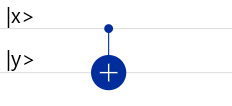
\includegraphics[scale=1]{cnot.png}
  \caption{CNot-Gatter}
  \label{fig:cnot}
\end{figure}

Im Verlauf dieser Arbeit werden einige kontrollierte Operationen verwendet. 
Für ein besseres Verständnis ist es hilfreich, 
sich diese Operationen mathematisch anzuschauen.
Die Transformation eines kontrollierten Pauli-X-Gatters lässt sich mit der folgenden Matrix beschreiben:
\[
  CX = 
  \begin{pmatrix}
    1 & 0 & 0 & 0\\
    0 & 1 & 0 & 0\\
    0 & 0 & 0 & 1\\
    0 & 0 & 1 & 0
    \end{pmatrix}
  \]
Um die Matrix mit den beiden Vektoren der beiden Qubits verrechnen zu können, 
wird das Tensorprodukt gebildet. Beispielsweise für \(\ket{xy}\) = \(\ket{10}\):
\[
  \begin{pmatrix}
    1 & 0 & 0 & 0\\
    0 & 1 & 0 & 0\\
    0 & 0 & 0 & 1\\
    0 & 0 & 1 & 0
    \end{pmatrix}
    \cdot
    \Bigg(
  \begin{pmatrix}
    0 \\
    1
  \end{pmatrix} \tensor
  \begin{pmatrix}
    1 \\
    0
  \end{pmatrix}
  \Bigg)
  =
  \begin{pmatrix}
    1 & 0 & 0 & 0\\
    0 & 1 & 0 & 0\\
    0 & 0 & 0 & 1\\
    0 & 0 & 1 & 0
    \end{pmatrix}
    \cdot
  \begin{pmatrix}
    0 \\
    0 \\
    1 \\
    0
  \end{pmatrix}
  =
  \begin{pmatrix}
    0 \\
    0 \\
    0 \\
    1
  \end{pmatrix}
  =
  \Bigg(
    \begin{pmatrix}
      0 \\
      1
    \end{pmatrix} \tensor
    \begin{pmatrix}
      0 \\
      1
    \end{pmatrix}
    \Bigg)
\]

Im Allgemeinen kann jedes Quanten-Gatter \(U\) als kontrolliertes Gatter eingesetzt werden. 
Dieses realisiert die Transformation~\cite{Hoever2023QC}: 
\[
  \text{für }
  U = 
  \begin{pmatrix}
    u_{00} & u_{01}\\
    u_{10} & u_{11}
    \end{pmatrix}
    \text{dementsprechend: }
    CU = 
  \begin{pmatrix}
    1 & 0 & 0 & 0\\
    0 & 1 & 0 & 0\\
    0 & 0 & u_{00} & u_{01}\\
    0 & 0 & u_{10} & u_{11}
    \end{pmatrix}
  \]


\subsubsection*{Aufeinander folgende Gatter} 

Um die Wirkung mehrerer Gatter zu berechnen, die nacheinander auf ein Qubit wirken, 
werden die Matrizen der Gatter in umgekehrter Reihenfolge aufgeschrieben, 
als diese im Quantenschaltkreis vorkommen. 
In Abbildung~\ref{fig:gate_order} wirkt zuerst ein Pauli-X-Gatter und anschließend ein Hadamard-Gatter auf das Qubit im Zustand \(\ket{0}\).
\[
  \frac{1}{\sqrt{2}}
  \begin{pmatrix}
    1 & 1 \\
    1 & -1
    \end{pmatrix} 
    \cdot
    \begin{pmatrix}
      0 & 1 \\
      1 & 0
      \end{pmatrix} 
    \cdot
    \begin{pmatrix}
      1  \\
      0 
      \end{pmatrix} 
      =
      \frac{1}{\sqrt{2}}
      \begin{pmatrix}
        1 & 1 \\
        1 & -1
        \end{pmatrix} 
      \cdot
      \begin{pmatrix}
        0  \\
        1 
        \end{pmatrix} 
        =
        \frac{1}{\sqrt{2}}
        \begin{pmatrix}
          1  \\
          -1 
          \end{pmatrix}
        =
        \ket{-}
  \]
\begin{figure}[H]
  \centering
  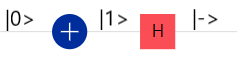
\includegraphics[scale=1]{gate_order.png}
  \caption{Berechnung aufeinanderfolgende Gatter}
  \label{fig:gate_order}
\end{figure}

\subsubsection*{Logische Gatter als Quantengatter} 
Das X-Gatter entspricht im Grunde genommen der identischen Transformation eines logischen NOT-Gatters für Basiszustände der Standardbasis.
\[
  X \cdot \ket{0} = \ket{1} 
  \text{ und }
  X \cdot \ket{1} = \ket{0}
\]
Quantengatter können die logischen Operatoren für zwei Bits, wie AND und XOR, 
nicht in ihrer herkömmlichen Form realisieren. 
Ein logisches AND als Quantengatter muss eines der beiden Qubits als Ergebnis der AND-Operation festlegen.
Im gegebenen Beispiel enthält das zweite Qubit das Ergebnis:
\[
  \ket{00} \shortrightarrow \ket{00} 
  \text{, } 
  \ket{01} \shortrightarrow \ket{00}
  \text{, }
  \ket{10} \shortrightarrow \ket{10}
  \text{, }
  \ket{11} \shortrightarrow \ket{11}
  \]
Unabhängig von der Definition des ersten Ausgangsqubits wird es immer zwei unterschiedliche Eingangszustände geben, 
die denselben Ausgangszustand haben. 

Es ist dennoch möglich, 
AND und OR als Quantengatter zu realisieren. 
Dafür muss ein Hilfsqubit verwendet werden, sodass das Quantengatter effektiv auf drei Qubits wirkt.

\subsection{Notation}
Die Notation von Quantenzuständen und Berechnungen ist in der Literatur nicht immer eindeutig. 
Um Mehrdeutigkeiten zu vermeiden, wird unter anderem die Schreibweise aus der Vorlesung "'Quanten Computing"` 
von Professor Hoever übernommen~\cite{Hoever2023QC}.

Dazu werden Qubits mit einem Index \(x\) versehen: \(\ket{\psi}_x\). 
Der Index gibt an, wie viele Qubits die Notation umfasst. 
Beispielsweise entspricht \(\ket{1}_1\) einem Qubit, 
welches sich im Zustand \(\ket{1}\) befindet.
Dank des Index ist bei den Qubits \(\ket{1}_3\) klar, 
dass es sich um drei Qubits handelt. 
Die Wertigkeit der Qubits wird durch die Reihenfolge festgelegt, 
dabei hat jedes Qubit den Wert einer Zweierpotenz.
Bei \(\ket{1}_3\) befinden sich die ersten beiden Qubits im Zustand \(\ket{0}\) und das Letzte im Zustand \(\ket{1}\).
Hingegen beschreibt \(\ket{4}_3\) ebenfalls drei Qubits, 
wobei diesmal das erste Qubit im Zustand \(\ket{1}\) ist und die letzten beiden dem Zustand \(\ket{0}\) entsprechen.
Also:
\[\ket{1}_3 = \ket{0}_1 \tensor \ket{0}_1 \tensor \ket{1}_1 = \ket{001}_3,~
\ket{4}_3 = \ket{1}_1 \tensor \ket{0}_1 \tensor \ket{0}_1 = \ket{100}_3\]

Ohne den Index 3 wäre die \(\ket{100}_3\) zweideutig. 
Der Index gibt an, dass es nur drei Qubits gibt. 
Da die dezimale 100 in binärer Schreibweise nicht mit drei Qubits darstellbar ist, 
muss es sich um die dezimale 4 handeln.

Zustände, die weder ein spezifisches Qubit noch ein Quantenregister beschreiben, 
werden ohne Index aufgeschrieben:
\[
  \ket{\psi}_1 = \alpha\ket{0} + \beta\ket{1}
  \]
Der Index wird auch ausgelassen, 
wenn ein Quantenregister einen Zustand beschreibt, 
der keine eindeutige Anzahl an Qubits vorschreibt.

\bigskip

Wenn mehrere gleiche Gatter parallel auf die identische Anzahl an Qubits angewendet werden 
oder das Gatter auf mehrere Qubits wirkt, 
wird das Gatter im Exponenten mit einem Tensor inklusive des Index beschrieben:
\[
  U^{\tensor x} \cdot 
  \ket{\psi}_x
\]


\subsection{Quanten-Fourier-Transformation} \label{Quanten-Fourier-Transformation}
Die Quanten-Fourier-Transformation bildet einen wesentlichen Bestandteil des implementierten Quantenalgorithmus. 
Im folgenden Abschnitt wird die allgemeine Anwendung der Quanten-Fourier-Transformation erklärt.
Darüber hinaus wird die Implementierung des Quantenschaltkreises anhand der Formel der Quanten-Fourier-Transformation hergeleitet.

Im Prinzip handelt es sich bei der Quanten-Fourier-Transformation um eine Transformation,
die Qubits von der Standardbasis (\(\ket{0}\), \(\ket{1}\)),
in die entsprechende Fourierbasis (\(\ket{+}\), \(\ket{-}\)) überführt~\cite[215]{homeister2023quantum215}.
Bei dem Basiswechsel werden die Informationen des vorherigen Zustands der Standardbasis in die Phase des neuen Zustandes übertragen~\cite{Ruiz-Perez2017}.
Anschließend können in der Fourierbasis Rechnungen durchgeführt werden, 
die im Grunde durch Manipulationen der Phase realisiert werden.
Mit diesem Ansatz ist es möglich, arithmetische Operationen, wie beispielsweise 
die Addition, effizienter zu berechnen~\cite{draper2000addition,Ruiz-Perez2017}.

Unter Verwendung der inversen Quanten-Fourier-Transformation, 
die als Rücktransformation dient, ist es möglich, 
wieder zurück in die Standardbasis zu transformieren. 
Dies ermöglicht die Extraktion der Information aus der Phase in einen messbaren Zustand.

Die Quanten-Fourier-Transformation ist für ein \(N\) = \(2^n\) mit \(n\) Qubits
für die Basisvektoren \(\ket{x}, x = 0,...,N-1\) wie folgt definiert~\cite[216]{homeister2023quantum215}:
\[QFT_{N}\ket{x}_{n} = \frac{1}{\sqrt{N}}\sum_{y=0}^{N-1}  e^{\frac{2 \pi i x y}{N}}\ket{y}_{n}\]
Anhand dieser Definition kann der Quantenschaltkreis nicht direkt hergeleitet werden.
Stattdessen muss die Formel umgeformt werden.

Die folgende Herleitung stammt aus dem Lehrbuch \textit{Quantum Computation and Quantum Information}~\cite[218]{nielsen_chuang_2010}.
Der Übersicht halber werden Zwischenschritte hinzugefügt.

Indem \(y\) in der ersten Formel in die Binärschreibweise überführt wird, ergibt sich:
\[ y = \sum_{k=1}^{n}2^{n-k} y_{n-k+1}\]  
\begin{align}
  QFT_{N}\ket{x}_{n} &=
    \frac{1}{\sqrt{N}}
    \sum_{y_n=0}^{1} ...
    \sum_{y_1=0}^{1} e^{\frac{2 \pi i x \sum_{k=1}^{n}2^{n-k} y_{n-k+1}}{N}}
    \ket{y_n ... y_{2}y_{1}}
\end{align}
Mit \(N\) = \(2^n\) kann der Bruch im Exponenten gekürzt werden:
\[QFT_{N}\ket{x}_{n} = \frac{1}{\sqrt{N}}\sum_{y_n=0}^{1}...\sum_{y_1=0}^{1}  e^{\frac{2 \pi i x \sum_{k=1}^{n}2^{n-k} y_{n-k+1}}{2^n}}\ket{y_n ... y_{2}y_{1}}\]
\[QFT_{N}\ket{x}_{n} = \frac{1}{\sqrt{N}}\sum_{y_n=0}^{1}...\sum_{y_1=0}^{1}  e^{2 \pi i x \sum_{k=1}^{n}2^{-k} y_{n-k+1}}\ket{y_n ... y_{2}y_{1}}\]
Anschließend kann der Ausdruck \(2^{-k}\) zu \(\frac{1}{2^k}\) umgeformt werden: 
\[QFT_{N}\ket{x}_{n} = \frac{1}{\sqrt{N}}\sum_{y_n=0}^{1}...\sum_{y_1=0}^{1}  e^{\frac{2 \pi i x \sum_{k=1}^{n} y_{n-k+1}}{2^k}}\ket{y_n ... y_{2}y_{1}}\]
Die Summe im Exponenten der Basis \(e\) kann als Produkt umgeschrieben werden.
Anstatt dem Produktzeichen \(\prod\) wird das Tensorprodukt \(\Tensor\) verwendet, da es sich um Qubits handelt:
\[QFT_{N}\ket{x}_{n} = \frac{1}{\sqrt{N}}\sum_{y_n=0}^{1}...\sum_{y_1=0}^{1} \Tensor_{k=1}^n{ e^{\frac{2 \pi i x y_k}{2^k}}}\ket{y_{k}}\]
Der Ausdruck kann weiter vereinfacht werden indem das Tensorprodukt vorgezogen wird:
\[QFT_{N}\ket{x}_{n} = \frac{1}{\sqrt{N}}\Tensor_{k=1}^n \Big[  \sum_{y_k=0}^{1}{ e^{\frac{2 \pi i x y_k}{2^k}}}\ket{y_{k}}\Big]\]
\[QFT_{N}\ket{x}_{n} = \frac{1}{\sqrt{N}}\Tensor_{k=1}^n \Big[  \ket{0} + { e^{\frac{2 \pi i x}{2^k}}}\ket{1}\Big]\] 
Schreibt man das Tensorprodukt voll aus und notiert \(x\) in Binärschreibweise, erhält man:
\begin{align*}
\frac{1}{\sqrt{N}}\Bigg(
  \Big(\ket{0} + { e^{\frac{2 \pi i (2^{n-1}x_n+...+2^1x_2+2^0x_1)}{2^1}}}\ket{1}\Big)
  &\tensor
  \Big(\ket{0} + { e^{\frac{2 \pi i (2^{n-1}x_n+...+2^1x_2+2^0x_1)}{2^2}}}\ket{1}\Big) \\
  &\vdotswithin{\tensor} \\
  &\tensor
  \Big(\ket{0} + { e^{\frac{2 \pi i (2^{n-1}x_n+...+2^1x_2+2^0x_1)}{2^n}}}\ket{1}\Big)
  \Bigg)
\end{align*}
Die komplexe Exponentialfunktion ergibt für eine natürliche Zahl \(k\): \(e^{2\pi i k} = 1\).
Mit dieser Eigenschaft kann man beispielsweise die Phasenverschiebung des ersten Tensors vereinfachen:
\begin{align*} 
  e^{\frac{2 \pi i (2^{n-1}x_n+ \dotsb +2^1x_2+2^0x_1)}{2^1}}
  &=
  e^{\frac{2 \pi i (2^{n-1}x_n)}{2^1}} \dotsb e^{\frac{2 \pi i (2^1x_2)}{2^1}} e^{\frac{2 \pi i (2^0x_1)}{2^1}} \\
  &=
  e^{{2 \pi i (2^{n-2}x_n)}} \dotsb e^{{2 \pi i (2^0x_2)}} e^{{2 \pi i (2^{-1}x_1)}}
\end{align*}
Dabei ergibt nur der Term \(e^{{2 \pi i (2^{-1}x_1)}} \neq 1 \)  
und verursacht somit eine relevante Phasenverschiebung.

Abschließend lässt sich das gesamte Tensorprodukt vereinfachen:
\begin{align*}
  QFT_{N}\ket{x}_{n} = 
  \frac{1}{\sqrt{N}}
  \Bigg(
    \Big(\ket{0} + { e^{\frac{2 \pi i (2^0x_1)}{2^1}}}\ket{1}\Big) 
    &\tensor
    \Big( \ket{0} + { e^{\frac{2 \pi i (2^1x_2+2^0x_1)}{2^2}}}\ket{1}\Big) \\
    &\vdotswithin{\tensor}\\
    &\tensor
    \Big( \ket{0} + { e^{\frac{2 \pi i (2^{n-1}x_n+ ... +2^1x_2+2^0x_1)}{2^n}}}\ket{1}\Big)
  \Bigg)
\end{align*}
Ein einzelner Tensor repräsentiert die Wirkung der Quantenschaltung auf ein einzelnes Qubit. 
Somit werden die Phasenverschiebungen erkennbar, 
die auf ein Qubit wirken. 
Außerdem verdeutlicht die Binärschreibweise, 
dass die angewendete Phasenverschiebung vom Zustand anderer Qubits abhängig sind.

Für die Implementierung der Quanten-Fourier-Transformation sind nur die Terme relevant, 
die eine Phasenverschiebung von ungleich 1 bewirken. 
Dies lässt sich mit der folgenden Formel beschreiben:
\[
QFT_{N}\ket{x}_{n} = \frac{1}{\sqrt{N}}
\Tensor_{k=1}^n \Big[  \ket{0} + { e^{\frac{2 \pi i \sum_{b=0}^{k-1}2^b x_{b+1} }{2^k}}}\ket{1}\Big]
\] 
Im Weiteren wird diese Formel verwendet, 
um einen Quantenschaltkreis für die Quanten-Fourier-Transformation mit drei Qubits zu implementieren:
\begin{align*}
QFT_{8}\ket{x}_{3} = 
\frac{1}{\sqrt{8}} 
  \Bigg[
    \Big(\ket{0} + { e^{\frac{2 \pi i (2^0x_1)}{2^1}}}\ket{1} \Big) 
    &\tensor
    \Big(\ket{0} + { e^{\frac{2 \pi i (2^1x_2+2^0x_1)}{2^2}}}\ket{1} \Big) \\
    &\tensor
    \Big(\ket{0} + { e^{\frac{2 \pi i (2^{2}x_3 +2^1x_2+2^0x_1)}{2^3}}}\ket{1} \Big) 
  \Bigg] 
\end{align*}
Man kann die durch den Eingangszustand eines einzelnen Qubits erzeugte Phasenverschiebung verdeutlichen, 
indem man die Addition im Exponenten zu einer Multiplikation der gleichen Basen umformt:
\begin{align*}
  QFT_{8}\ket{x}_{3} = 
  \frac{1}{\sqrt{8}} 
  \Bigg[
    \Big(\ket{0} + { e^{\frac{2 \pi i (2^0x_1)}{2^1}}}\ket{1}\Big) 
    &\tensor
    \Big(\ket{0} + { e^{\frac{2 \pi i (2^1x_2)}{2^2}} e^{\frac{2 \pi i (2^0x_1)}{2^2}} }\ket{1} \Big) \\ 
    &\tensor
    \Big(\ket{0} + { e^{\frac{2 \pi i (2^{2}x_3)}{2^3}} e^{\frac{2 \pi i (2^1x_2)}{2^3}} e^{\frac{2 \pi i (2^0x_1)}{2^3}}  }\ket{1} \Big)
  \Bigg] 
\end{align*}
Die wirkenden Phasenverschiebungen werden eindeutiger, 
indem man die Brüche kürzt:
\begin{align*}
  QFT_{8}\ket{x}_{3} = 
  \frac{1}{\sqrt{8}} 
  \Bigg[ 
    \Big( \ket{0} + e^{\pi i x_1}\ket{1} \Big) &\tensor
    \Big(\ket{0} + { e^{\pi i x_2} e^{ \frac{ \pi i x_1}{2}} }\ket{1} \Big) \\ &\tensor
    \Big(\ket{0} + { e^{\pi i x_3} e^{\frac{\pi i x_2}{2}} e^{ \frac{ \pi i x_1}{4}} }\ket{1} \Big) 
  \Bigg] 
\end{align*}
In einer abschließenden Umformung lässt sich der Bruch \(\frac{1}{\sqrt8}\) aufteilen.
Dadurch erinnern die einzelnen Tensoren,
beziehungsweise Qubits an die Form die durch eine Hadamard-Transformation entsteht:
\begin{align*}
  QFT_{8}\ket{x}_{3} = 
   \frac{1}{\sqrt{2}}\Big( \ket{0} + e^{\pi i x_1}\ket{1} \Big) 
   &\tensor
  \frac{1}{\sqrt{2}}\Big( \ket{0} + { e^{\pi i x_2} e^{ \frac{ \pi i x_1}{2}} }\ket{1} \Big) \\ 
  &\tensor
  \frac{1}{\sqrt{2}}\Big( \ket{0} + { e^{\pi i x_3} e^{\frac{\pi i x_2}{2}} e^{ \frac{ \pi i x_1}{4}} }\ket{1} \Big)  
\end{align*}
Die Phasenverschiebung \(e^{\pi i}\) ist in jedem der einzelnen Qubits vorhanden.
Des Weiteren ist diese Phasenverschiebung von dem Eingangszustand des Qubits abhängt,
auf das die Verschiebung auch angewendet wird. 
Konkret bedeutet dies, 
dass auf jedes Qubit in dem Zustand \(\ket{1}\) eine Phasenverschiebung von \(e^{\pi i}\) wirkt.
Anhand des ersten Qubits, 
beziehungsweise des ersten Tensors, 
ergibt sich bei \(x_1 = 0\)
der Zustand: 
\[\frac{1}{\sqrt{2}}(\ket{0} + e^{\pi i 0} \ket{1}) = \frac{1}{\sqrt{2}}(\ket{0} + \ket{1})\]
Bei \(x_1 = 1\) wird der Zustand zu:
\[\frac{1}{\sqrt{2}}(\ket{0} + e^{\pi i 1} \ket{1}) = \frac{1}{\sqrt{2}}(\ket{0} - \ket{1})\]
Aufgrund des Vorfaktors von \(\frac{1}{\sqrt{2}}\) entsprechen beide Fälle also der Hadamard"=Transformation.
Da alle anderen Tensoren ebenfalls den Ausdruck \(e^{\pi i x_k}\) 
und den Vorfaktor \(\frac{1}{\sqrt{2}}\) beinhalten, 
wirkt auf jedes Qubit ein Hadamard-Gatter.

Die weiteren Tensoren des Tensorprodukts beinhalten zunehmend mehr Ausdrücke, 
die für unterschiedliche Phasenverschiebungen sorgen. 
Die Phasenverschiebung eines einzelnen Ausdrucks kann mit einem Phasen-Gatter realisiert werden. 

Beispielsweise wirkt auf das zweite Qubit ein Phasen-Gatter mit \(P(\frac{\pi}{2} )\).
Diese Phasenverschiebung soll jedoch nur angewendet werden, 
wenn \(x_1 = 1\) ist.
Aus diesem Grund wird das Phasen-Gatter durch den Eingangszustand des ersten Qubits gesteuert und 
mithilfe eines kontrollierten Phasen-Gatters realisiert.
Das gleiche Prinzip gilt für alle weiteren Qubits.
Anschließend ergibt sich ein Quantenschaltkreis, 
wie dieser in Abbildung~\ref{fig:qft} dargestellt ist.

Wie in Abbildung~\ref{fig:qft} ersichtlich, 
kehrt die Quanten-Fourier-Transformation die Reihenfolge der Qubits um~\cite[217]{homeister2023quantum215}.
Um die ursprüngliche Reihenfolge wiederherzustellen, 
werden am Ende der Quanten-Fourier-Transformation Swap-Operationen durchgeführt.
\begin{figure}[H]
  \centering
  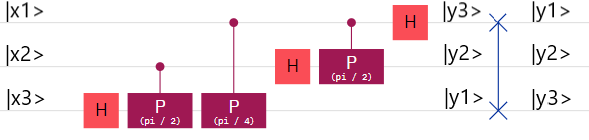
\includegraphics[width=\columnwidth]{qft.PNG}
  \caption{3-Qubit QFT}
  \label{fig:qft}
\end{figure}

Anhand der Implementierung wird ersichtlich,
dass die Quanten-Fourier-Transformation unitär ist. 
Diese Eigenschaft ergibt sich aus der Tatsache, 
dass der zugehörige Quantenschaltkreis ausschließlich unter Verwendung von unitären Gattern realisierbar ist.

Wie bereits oben erwähnt, 
wird für die Rücktransformation aus der Fourierbasis in die Standardbasis die inverse Quanten-Fourier-Transformation angewendet.
Um einen Quantenschaltkreis aus unitären Gattern zu invertieren, 
werden die Inversen der verwendeten Gatter in umgekehrter Reihenfolge zur ursprünglichen Schaltung angewendet. 
Die Swap-Operationen stehen somit bei der inversen Quanten-Fourier-Transformation am Anfang.
In Abbildung~\ref{fig:iqft} ist beispielhaft die inverse Quanten-Fourier-Transformation für drei Qubits abgebildet.
\begin{figure}[H]
  \centering
  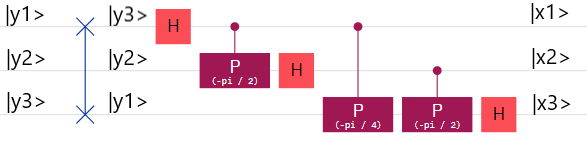
\includegraphics[width=\columnwidth]{iqft.PNG}
  \caption{3-Qubit inverse QFT}
  \label{fig:iqft}
\end{figure}

\subsection{Quantum-Phase-Estimation} \label{Quanten-Phase-Estimation}

Im nachfolgenden Abschnitt wird die Anwendung und Funktionsweise des Quantum-Phase-Estimation Quantenalgorithmus erläutert. 
Die Quantum-Phase-Estimation ist ein Bestandteil einiger fortgeschrittener Quantenalgorithmen und eine integrale Komponente des spezifischen Quantenalgorithmus, 
der in dieser Arbeit implementiert wird. 
Genauer gesagt, 
basiert der implementierte Quantenalgorithmus auf den Prinzipien der Quantum-Phase-Estimation und verwendet dieselbe Methodik für einen spezialisierten Kontext.

Schwerpunktmäßig konzentriert sich die Erklärung primär auf das Verständnis der Funktionsweise der Quantum-Phase-Estimation.
Die Anwendung der Quantum-Phase-Estimation benötigt ein paar Voraussetzungen die vom spezifischen Kontext abhängen, 
in dem die Quantum-Phase-Estimation angewendet wird.
Die Voraussetzungen werden für die Erklärung der Funktionsweise als Gegeben angesehen.

Im weiteren Verlauf der Arbeit werden diese Voraussetzungen im Hinblick auf den Anwendungsfall des implementierten Quantenalgorithmus konkretisiert.

Eine der Voraussetzungen ist, 
dass ein Eigenvektor \(\ket{x}_n\) einer unitären Transformation \(U^{\tensor n}\) bekannt ist.
Wendet man die Transformation \(U^{\tensor n}\) auf \(\ket{x}_n\) an, 
so gilt~\cite[221]{nielsen_chuang_2010}: 
\[U^{\tensor n}\ket{x}_n=\lambda_x\ket{x}_n\]
Dabei erhält man, abhängig vom gewählten Eigenvektor \(\ket{x}_n\), einen der Eigenwert \(\lambda_x\) von \(U^{\tensor n}\).
Ein Eigenwert \(\lambda_x\) besitzt die Form eines Phasenfaktors: \(e^{2\pi i \varphi_x}\),
mit \(0 \leq \varphi_x < 1\).
Im Prinzip wird durch die unitäre Transformation also eine globale Phasenverschiebung auf den Eigenvektor angewendet.

Wie bereits im Kapitel zu den Grundlagen gezeigt wurde, 
ist es nicht möglich, eine globale Phase durch eine gewöhnliche Messung der Qubits zu bestimmen. 
Das liegt daran, dass eine globale Phase die Amplituden eines Qubits nicht verändert und 
somit die Wahrscheinlichkeiten der Messergebnisse unverändert bleiben. 
Stattdessen muss man die Qubits so manipulieren, 
dass die globale Phase doch Einfluss auf die Amplituden nimmt.

Der Quantum-Phase-Estimation Quantenalgorithmus ist in der Lage, 
den Eigenwert aus \(U^{\tensor n}\ket{x}_n=\lambda_x\ket{x}_n\), 
also die Phasenverschiebungen repräsentiert durch \(\lambda_x = e^{2\pi i \varphi_x}\),
auf die Amplitude eines anderen Qubits zu verschieben.
Um \(\lambda_x\) auf ein anderes Qubit zu übertragen, 
wird der Effekt des \emph{Phase-Kickback} genutzt.
Anschließend wird der Wert \(\varphi_x\) des Eigenwertes durch die inverse Quanten-Fourier-Transformation in einen messbaren Zustand überführt.

Der Phase-Kickback tritt auf, 
wenn eine unitäre Transformation \(U^{\tensor n}\), die durch ein Qubit \(\ket{y}_1\) in Superposition kontrolliert wird,
auf einen Eigenvektor \(\ket{x}_n\) von \(U^{\tensor n}\) anwendet wird.
Dabei wird der Eigenwert, genauer gesagt \(\lambda_x\), 
auf den \(\ket{1}\)-Anteil von \(\ket{y}_1\) übertragen.

Sei \( \ket{y}_1 = \alpha\ket{0} + \beta\ket{1} \) mit \( \alpha,\beta \neq 0 \), dann gilt:
\begin{align*}
  CU^{\tensor n+1}(\ket{y}_1 \otimes \ket{x}_n) 
  &= CU^{\tensor n+1}\big((\alpha\ket{0} + \beta\ket{1}) \otimes \ket{x}_n\big) \\
  &= CU^{\tensor n+1}\big((\alpha\ket{0}\otimes\ket{x}_n) + (\beta\ket{1}\otimes \ket{x}_n)\big) \\
  &= \big((\alpha\ket{0}\otimes\ket{x}_n) + (\beta\ket{1}\otimes U^{\tensor n}\ket{x}_n)\big) \\
  &= \big((\alpha\ket{0}\otimes\ket{x}_n) + (\beta\ket{1}\otimes \lambda_x\ket{x}_n)\big) \\
  &= (\alpha\ket{0} + \lambda_x\beta\ket{1}) \otimes \ket{x}_n
\end{align*}
In der Rechnung wird also die globale Phase \(\lambda_x\) von \(\ket{x}_n\) als relative Phase auf \(\ket{y}_1\) übertragen.

Es folgt ein Beispiel welches den Effekt verdeutlicht:
Beachtet werden zwei Qubits im Zustand \(\ket{+}_1 \tensor \ket{-}_1\) auf die ein kontrolliertes X-Gatter angewendet wird.
Dabei ist \(\ket{-}_1\) der Eigenvektor einer X-Transformation mit zugehörigen Eigenwert \(e^{\pi i} = -1\), also: 
\[X \cdot \ket{-}_1=-\ket{-}_1\]
Auf das zweite Qubit \(\ket{-}_1\) wirkt ein \(CX^{\tensor 2}\) Gatter welches durch das erste Qubit \(\ket{+}_1\) kontrolliert wird:
\[
  CX^{\tensor 2}( \ket{+}_1\ \tensor \ket{-}_1) =
  \begin{pmatrix}
    1 & 0 & 0 & 0\\
    0 & 1 & 0 & 0\\
    0 & 0 & 0 & 1\\
    0 & 0 & 1 & 0
  \end{pmatrix}
  \cdot
  \frac{1}{{2}}
  \begin{pmatrix}
    1 \\
    -1 \\
    1 \\
    -1 
  \end{pmatrix}
  =
  \frac{1}{{2}}
  \begin{pmatrix}
    1 \\
    -1 \\
    -1 \\
    1 
  \end{pmatrix}
  \]
  \[
  =
  \frac{1}{{\sqrt{2}}}
  \begin{pmatrix}
    1 \\
    -1 
  \end{pmatrix}
  \tensor
  \frac{1}{{\sqrt{2}}}
  \begin{pmatrix}
    1 \\
    -1 
  \end{pmatrix}
  =
  \ket{-}_1 \tensor \ket{-}_1
  \]
Mit Hilfe des Phase-Kickback kann man also den Eigenwert einer unitären Transformation in die relative Phase eines Kontrollqubits verschieben.
Der Vorteil davon ist, 
dass diese Phasenverschiebung nur den Vorfaktor von \(\ket{1}\) des Kontrollqubits betrifft und keine globale Phase darstellt.

Der Aufbau einer Quantum-Phase-Estimation Quantenschaltung sieht beispielsweise wie folgt aus:
Beachtet wird die unitäre Transformation eines Phase-Gatters(P) mit einer variablen Phasenverschiebung von 
\[P(2 \pi \varphi ) = 
\begin{pmatrix}
  1 & 0\\
  0 & e^{2 i \pi \varphi}
\end{pmatrix}\]
Ein zugehöriger Eigenvektor dieser Transformation ist \(\ket{1}_1\), 
den: 
\[P(2 \pi \varphi)\ket{1}_1 = e^{2 i \pi \varphi} \ket{1}_1\]

Um den Effekt des Phase-Kickback nutzen zu können, 
muss sich das Kontrollqubit in einer Superposition befinden.
Dafür wird das Kontrollqubit im Zustand \(\ket{0}_1\) initialisiert und
anschließend mit einem Hadamard-Gatter(H) in die gleichmäßige Superposition \(\ket{+}_1\) versetzt.
\[\ket{0}_1 \tensor \ket{1}_1 
\underrightarrow{H^{\tensor 1}}
 \ket{+}_1 \tensor \ket{1}_1
=
\frac{1}{\sqrt{2}}
\begin{pmatrix}
  1 \\
  1
 \end{pmatrix}
 \tensor
 \begin{pmatrix}
  0 \\
  1 
 \end{pmatrix}
 =
 \frac{1}{\sqrt{2}}
 \begin{pmatrix}
  0 \\
  1 \\
  0 \\
  1
\end{pmatrix}
 \]
Über das kontrollierte Phase-Gatter wird der Eigenwert auf das Kontrollqubit verschoben und
befindet sich daher nicht mehr im Zustand \(\ket{+}_1\) :
\begin{align*}
  \frac{1}{\sqrt{2}}
  \begin{pmatrix}
   0 \\
   1 \\
   0 \\
   1
  \end{pmatrix}
  \underrightarrow{CP^{\tensor 2}(2 \pi \varphi)}
  \begin{pmatrix}
    1 & 0 & 0 & 0\\
    0 & 1 & 0 & 0\\
    0 & 0 & 1 & 0\\
    0 & 0 & 0 & e^{2 i \pi \varphi}
  \end{pmatrix}
  \cdot
  \frac{1}{\sqrt{2}}
  \begin{pmatrix}
   0 \\
   1 \\
   0 \\
   1
  \end{pmatrix}
  &=
  \frac{1}{\sqrt{2}}
  \begin{pmatrix}
    0 \\
    1 \\
    0 \\
    e^{2 i \pi \varphi}
  \end{pmatrix} \\
  &=
  \frac{1}{\sqrt{2}}
  \begin{pmatrix}
    1 \\
    e^{2 i \pi \varphi}
   \end{pmatrix}
   \tensor
   \begin{pmatrix}
    0 \\
    1 
   \end{pmatrix}
\end{align*}
Anschließend wird auf die Kontrollqubits die inverse Quanten-Fourier-Transformation angewendet.
Die inverse Quanten-Fourier-Transformation sorgt dafür, 
dass der Eigenwert die Amplituden der Kontrollqubits beeinflusst.
Die Qubits mit dem Eigenvektor sind für den weiteren Ablauf der Quantum-Phase-Estimation nicht mehr relevant 
und werden nicht weiter beachtet.
Im vorliegenden Beispiel entspricht die inverse Quanten-Fourier-Transformation einem einzelnen Hadamard-Gatter. 
Das liegt daran, dass lediglich ein Kontrollqubit vorhanden ist, 
auf das die inverse Quanten-Fourier-Transformation angewendet wird:
\[
\frac{1}{\sqrt{2}}
\begin{pmatrix}
  1 \\
  e^{2 i \pi \varphi}
 \end{pmatrix}
 \underrightarrow{H^{\tensor 1}}
 \frac{1}{\sqrt{2}}
 \begin{pmatrix}
  1 & 1\\
  1 & -1
 \end{pmatrix}
 \cdot
 \frac{1}{\sqrt{2}}
\begin{pmatrix}
  1 \\
  e^{2 i \pi \varphi}
 \end{pmatrix}
 =
 \frac{1}{2}
 \begin{pmatrix}
  1 + e^{2 i \pi \varphi}\\
  1 - e^{2 i \pi \varphi}
 \end{pmatrix}
\]
Das Ergebnis des Beispiels zeigt, dass der Eigenwert praktisch auf die Amplitude vom Kontrollqubit transformiert wird.

Verwendet man ein Phase-Gatter mit \(\varphi  = 0.075\), 
so sieht der Quantenschaltkreis wie in Abbildung~\ref{fig:qpe_1qubit} aus.
\begin{figure}[H]
  \centering
  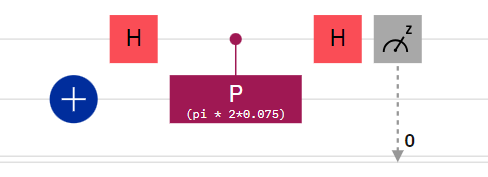
\includegraphics[ scale = 0.9]{qpe_1qubit.PNG}
  \caption{Einzelnes Kontroll-Qubit QPE}
  \label{fig:qpe_1qubit}
\end{figure}
Mit dieser Phasenverschiebung sollte man bei einer Messung den Zustand \(\ket{0}\)
mit einer Wahrscheinlichkeit von ungefähr \(0.9455\) 
und den Zustand \(\ket{1}\) mit der Wahrscheinlichkeit \(0.0544\) erhalten.
Die Ergebnisse von 20.000 Messungen, dargestellt in Abbildung~\ref{fig:qpe_1qubit_Messung}, 
bestätigen die Größenordnung dieser Wahrscheinlichkeiten.
Jedoch entsprechen die Messungen aus Abbildung~\ref{fig:qpe_1qubit_Messung} nicht ganz den theoretisch ausgerechneten Wahrscheinlichkeiten.
Dies liegt an der probabilistischen Natur der Messung.
Bei einer zunehmenden Anzahl an Messungen würden die Ergebnisse gegen die theoretisch erwarteten Wahrscheinlichkeitswerte konvergieren.
Somit sind viele Durchläufe des Quantenalgorithmus erforderlich, 
um anhand der Messungen ein verlässliches Ergebnis zu erhalten.
\begin{figure}[H]
  \caption{Einzelnes Kontroll-Qubit QPE Messung}
  \label{fig:qpe_1qubit_Messung}
  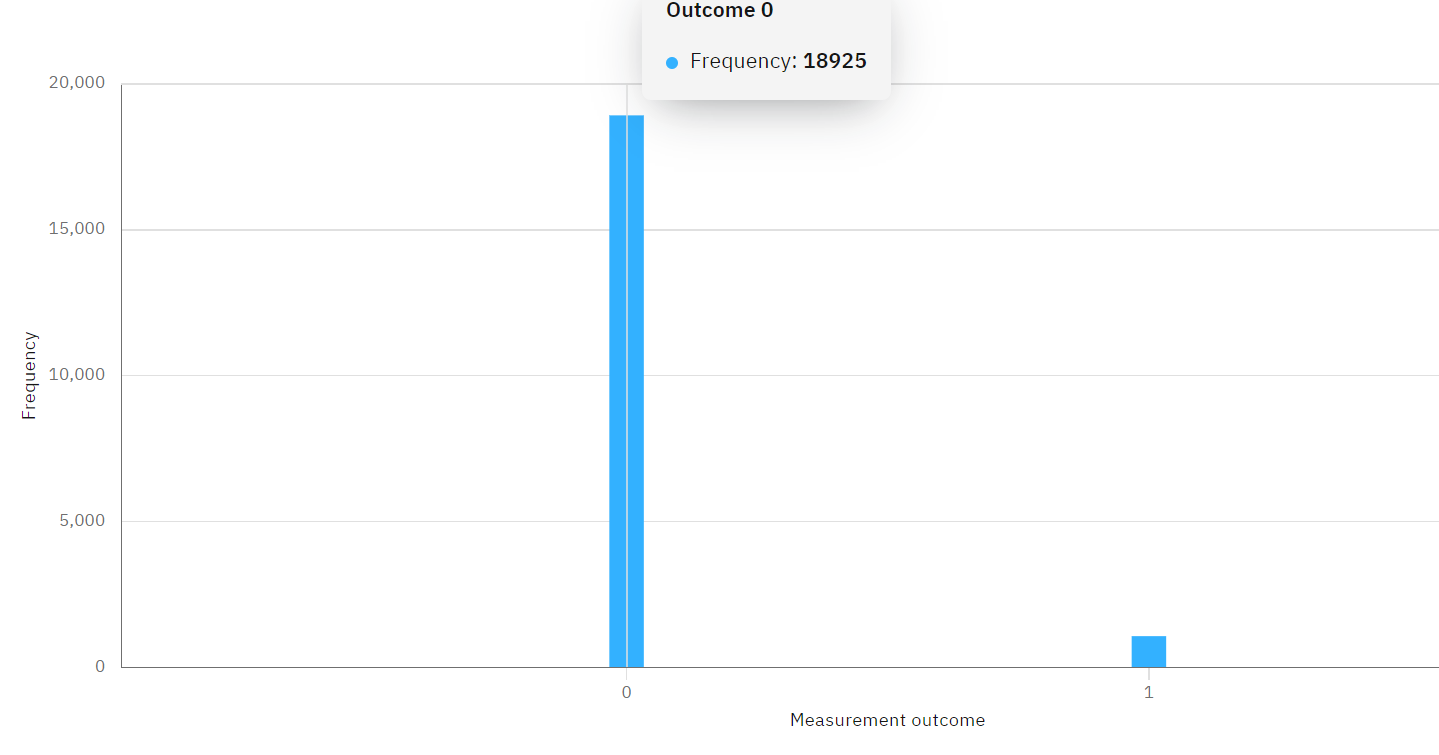
\includegraphics[width=\columnwidth]{qpe_1qubit_Messung.PNG}
  \centering
  \end{figure}
  

Die Präzision der Quantum-Phase-Estimation lässt sich durch die Verwendung mehrerer Qubits erhöhen.
Diese zusätzlichen Qubits dienen als weitere Kontrollqubits.
Die Anzahl der Qubits, die für den Eigenvektor benötigt werden, 
bleibt unverändert und entspricht der Bitanzahl, 
die ausreicht, um den Wert des Eigenvektors zu definieren.
Jedes einzelne Kontrollqubit kontrolliert ein \(U^{2^x}\)-Gatter.
Bei \(n\) Kontrollqubits kontrolliert das least-significant-bit ein \(U^{2^0}\)-Gatter,
das darauffolgende ein \(U^{2^1}\)-Gatter und so weiter,
bis das letzte Kontrollqubit ein \(U^{2^{n-1}}\)-Gatter kontrolliert.
\(U^{2^x}\) kann entweder durch \(2^x\) viele \(U\)-Gatter oder durch ein einzelnes Gatter implementiert werden, 
das den Eigenwert \(\lambda\) mit \(2^x\) multipliziert anwendet.
Anschließend wird die inverse Quanten-Fourier-Transformation auf alle Kontrollqubits angewendet.
Durch die Messung lässt sich dann der Wert für \(\varphi\) ermitteln.
Der Aufbau der Schaltung ist als Skizze in Abbildung~\ref{fig:qpe_n_qubit} abgebildet.

\begin{figure}[H]
  \centering
  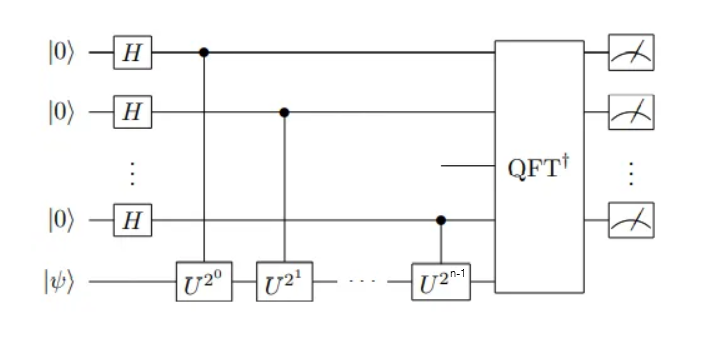
\includegraphics[scale = 0.8]{qpe_n_qubit.PNG}
  \caption{N Qubit QPE}
  \label{fig:qpe_n_qubit}
\end{figure}

Wird die Quanten-Fourier-Transformation wie in Abbildung~\ref{fig:qpe_n_qubit} realisiert,
kann man den Zustand der Kontrollqubits vor der inversen Quanten-Fourier-Transformation wie folgt beschreiben:
\[\frac{1}{\sqrt{N}}\Bigg[
  CU^{2^0}\Big(\ket{0} + \ket{1}\Big) \tensor
  CU^{2^1}\Big(\ket{0} + \ket{1}\Big) \tensor 
  ... \tensor
  CU^{2^{n-1}}\Big(\ket{0} + \ket{1}\Big) 
  \Bigg]\]
Mit \(U^{2^x}\ket{x}_n=e^{2\pi i 2^x\varphi}\ket{x}_n\) wird der Eigenwert \(e^{2\pi i \varphi}\) wegen des Phase-Kickbacks
über die \(CU\)-Gatter auf die Kontrollqubits übertragen:
\[\frac{1}{\sqrt{N}}\Bigg[
  \Big(\ket{0} + e^{2\pi i 2^0 \varphi}\ket{1}\Big) \tensor
  \Big(\ket{0} + e^{2\pi i 2^1 \varphi}\ket{1}\Big) \tensor 
  ... \tensor
  \Big(\ket{0} + e^{2\pi i 2^{n-1} \varphi}\ket{1}\Big) 
  \Bigg]\]
Schreibt man \(\varphi\) als Binärbruch:
\[\varphi = \frac{\varphi_n}{2^1} + \frac{\varphi_{n-1}}{2^2} + ... + \frac{\varphi_1}{2^n}\]
Kann die Formel in einer ähnlichen Form wie die Quanten-Fourier-Transformation umgeformt werden:
\begin{align*}
\frac{1}{\sqrt{N}}\Bigg[
  \Big(\ket{0} + e^{2\pi i (\frac{\varphi_n}{2})} 
  ...  
  e^{2\pi i (\frac{\varphi_2}{2^{n-1}})}e^{2\pi i (\frac{\varphi_1}{2^{n}})}\ket{1}\Big) 
  \tensor ... 
  &\tensor
  \Big(\ket{0} +  e^{2\pi i (\frac{\varphi_2}{2})}e^{2\pi i (\frac{\varphi_1}{4})}\ket{1}\Big)\\ 
  &\tensor 
  \Big(\ket{0} + e^{2\pi i (\frac{\varphi_1}{2})}\ket{1}\Big) 
  \Bigg]
\end{align*}
Die Formel besitzt die gespiegelte Struktur wie die Quanten-Fourier-Transformation ohne Swap-Gatter:
\begin{align*}
  QFT_{N}\ket{x}_{n} = 
  \frac{1}{\sqrt{N}}
  \Bigg[
    \Big(\ket{0} + { e^{2 \pi i (\frac{x_1}{2})}}\ket{1}\Big) 
    &\tensor
    \Big( \ket{0} + { e^{2 \pi i (\frac{x_2}{2})(\frac{x_1}{4})}}\ket{1}\Big)\\
    &\vdotswithin{\tensor}\\
    &\tensor
    \Big(\ket{0} + e^{2\pi i (\frac{x_n}{2})} ... e^{2\pi i (\frac{x_2}{2^{n-1}})}e^{2\pi i (\frac{x_1}{2^{n}})}\ket{1}\Big)
  \Bigg]
\end{align*}
Durch die Verwendung der Swap-Gatter kann die Reihenfolge der Quanten-Fourier-Transformation gespiegelt werden, 
anschließend sind beide Formeln strukturell identisch.

Wie im Abschnitt zur Quanten-Fourier-Transformation erklärt,
transformiert die Quanten-Fourier-Transformation den Zustand der Eingangsqubits \(\ket{x}_n\) in die Phasen der Ausgangsqubits.
Im Gegensatz dazu kehrt die inverse Quanten-Fourier-Transformation diesen Vorgang um, 
indem die Phaseninformationen der Eingangsqubits in Zustände der Standardbasis transformiert werden.

Die Anwendung der inversen Quanten-Fourier-Transformation, inklusive Swap-Gatter, bewirkt also:
\begin{align*}
iQFT\Bigg(
\frac{1}{\sqrt{N}}
\Bigg[
  \Big(\ket{0} + e^{2\pi i (\frac{\varphi_n}{2})} ...& e^{2\pi i (\frac{\varphi_2}{2^{n-1}})}e^{2\pi i (\frac{\varphi_1}{2^{n}})}\ket{1}\Big) \\
  &\vdotswithin{\tensor}\\
  &\tensor
  \Big(\ket{0} +  e^{2\pi i (\frac{\varphi_2}{2})}e^{2\pi i (\frac{\varphi_1}{4})}\ket{1}\Big) \tensor 
  \Big(\ket{0} + e^{2\pi i (\frac{\varphi_1}{2})}\ket{1}\Big) 
  	\Bigg]
\Bigg)
\end{align*}
\[ = \ket{\varphi_1 \varphi_{2}...\varphi_n}_n = \ket{2^n\varphi}_n\]
Schließlich kann \(\varphi\) mit einer Division durch \(2^n\) bestimmt werden.

Als Beispiel wird die Quantum-Phase-Estimation für
\(U\ket{1}_1=e^{2\pi i \frac{3}{8}}\ket{1}_1\), 
also mit \(\varphi = \frac{3}{8}\) betrachtet.
Im Quantenschaltkreis aus Abbildung~\ref{fig:3_qubit_qpe} 
werden die kontrollierten \(U^{2^x}\)-Gatter als Phase-Gatter mit steigendem \(x\) in \(P(2^x 2\pi \frac{3}{8})\) realisiert.
\begin{figure}[H]
  \centering
  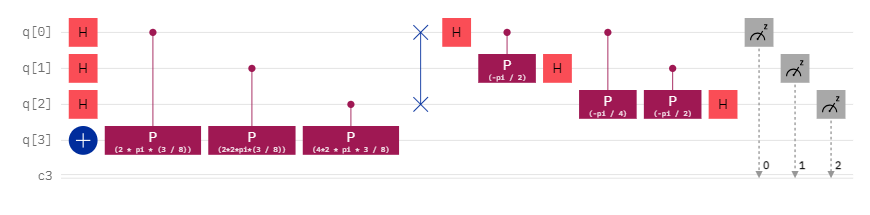
\includegraphics[width=\columnwidth]{3_qubit_qpe.png}
  \caption{3-Kontroll-Qubit QPE}
  \label{fig:3_qubit_qpe}
\end{figure}
Die Messung in Abbildung~\ref{fig:3_qubit_qpe_measurement} ergibt konsistent bei allen Durchläufen den Zustand \(\ket{3}_3\).
Da \(\ket{3}_3 = \ket{2^3\varphi}_3\) entspricht, 
lässt sich durch eine Division \(\varphi = \frac{3}{8}\) ermitteln.
Es ist zu beachten, 
dass die Reihenfolge der Wertigkeit der Qubits gleich bleibt.
Normalerweise tauschen die inverse wie auch die normale Quanten-Fourier-Transformation die Wertigkeiten.
Dieser Effekt wird jedoch durch Swap-Gatter korrigiert.
\begin{figure}[H]
  \centering
  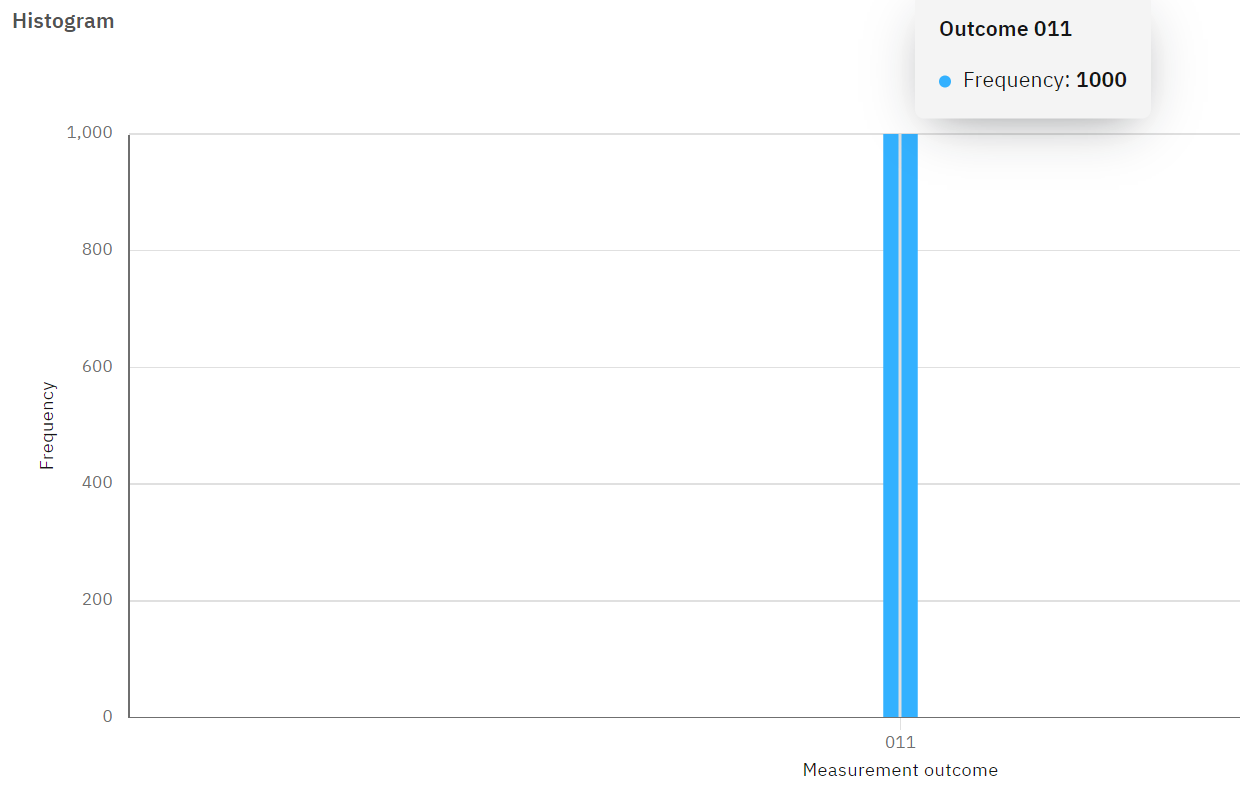
\includegraphics[width=\columnwidth]{3_qubit_qpe_measurement.PNG}
  \caption{3-C-Qubit QPE Messergebnis}
  \label{fig:3_qubit_qpe_measurement}
\end{figure}

Im vorherigen Beispiel liefern die Messungen aller Durchläufe den gleichen Zustand, 
mit dem \(\varphi\) eindeutig bestimmbar ist.
Diese Eindeutigkeit tritt auf, 
wenn die verwendete Anzahl an Kontroll-Qubits ausreicht, 
um \(\varphi\) eindeutig zu repräsentieren.
Im obigen Beispiel kann \(\varphi\) eindeutig mit den drei verwendeten Kontrollqubits dargestellt werden:
\[{\frac{3}{8} =0 \cdot 2^{-1} + 1\cdot2^{-2} + 1\cdot2^{-3}}\]
Verwendet man nicht ausreichend Kontroll-Qubits, 
kann \(\varphi\) nicht eindeutig repräsentiert werden.
Als Konsequenz wird die Messung ungenau.
Mit hoher Wahrscheinlichkeit kollabieren die Qubits bei einer Messung 
in die darstellbaren Zustände, 
die den genauen Wert am besten approximieren.
Dabei liegt die Wahrscheinlichkeit, dass die Messung in einen der beiden angrenzenden Zustände kollabiert, 
bei mindestens \(\frac{8}{\pi^2}\)~\cite[119]{kaye2007introduction}.

In Abbildung~\ref*{fig:3_qubit_qpe_measurment_uncertain} sind die Messergebnisse einer Quantum-Phase-Estimation abgebildet, 
die die Phase \(\varphi = \frac{5}{16}\) bestimmen soll.
Da \(\frac{5}{16}\) nicht mit 3 Qubits darstellbar ist, 
gibt es kein eindeutiges Messergebnis.
Anhand der Messergebnisse ist aber erkennbar, 
dass die Messungen mit einer Wahrscheinlichkeit größer als \(\frac{8}{\pi^2}\) in
einen der beiden angrenzenden Zustände kollabiert.
Diese entsprechen \({\frac{2}{8} = \frac{4}{16}}\) und \({\frac{3}{8} = \frac{6}{16}}\), 
also genau den Werten, die \(\frac{5}{16}\) am nächsten sind.

\begin{figure}[H]
  \centering
  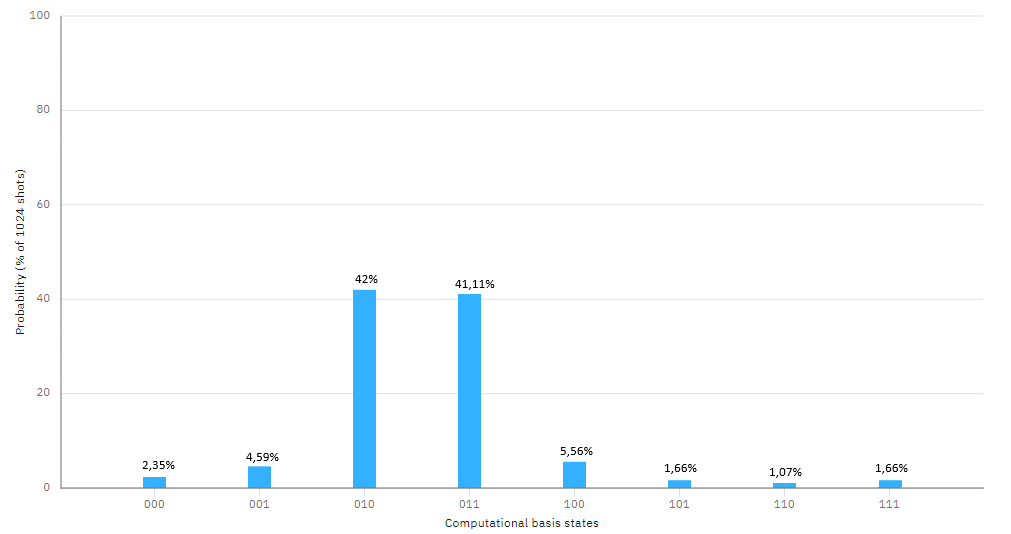
\includegraphics[width=\columnwidth]{3_qubit_qpe_measurment_uncertain.PNG}
  \caption{QPE unpräzises Messergebnis}
  \label{fig:3_qubit_qpe_measurment_uncertain}
\end{figure}












 






 











